\documentclass[table]{beamer}
\usepackage[utf8]{inputenc}
\usepackage{xcolor}
\usepackage{tcolorbox}
\usepackage{adjustbox}
\usepackage{multicol}
\usepackage{multirow}
\usepackage{eurosym}
\usepackage{amsmath}
\usepackage{ragged2e}
\usepackage[scaled]{helvet}
\usepackage{tikz}
\usetikzlibrary{spy,shapes,arrows,positioning,decorations.pathreplacing}

\tikzset{hide on/.code={\only<#1>{\color{white}}}}
\definecolor{dark_green}{rgb}{0.0, 0.5, 0.0}

\pgfdeclarelayer{bg}    % declare background layer
\pgfsetlayers{bg,main}  % set the order of the layers (main is the standard layer)

\apptocmd{\frame}{}{\justifying}{}

\definecolor{iscal_color}{HTML}{641242} % ISCAL

\setbeamertemplate{footline}{
	\hspace{0.05\textwidth}
	\raisebox{3ex}{\insertshortauthor{}}\hfill
	\raisebox{3ex}{\insertframenumber{}/\inserttotalframenumber} \hfill
	{
\includegraphics[height=0.08\textheight]{../visual material/logo.png}}
	\hspace{0.05\textwidth}
}

\tikzset{
  invisible/.style={opacity=0},
  visible on/.style={alt={#1{}{invisible}}},
  alt/.code args={<#1>#2#3}{%
    \alt<#1>{\pgfkeysalso{#2}}{\pgfkeysalso{#3}} % \pgfkeysalso doesn't change the path
  },
}

\title{Microeconomia}
\subtitle{Capitulo 1 : Princ\'ipios fundamentais}
\author[]{}
\institute[ISCAL]{
\includegraphics[height=0.10\textheight]{../visual material/logo_eng_full.png}}
\date{Primavera 2020/2021}

\setbeamertemplate{navigation symbols}{}

\setbeamercolor{title}{fg = iscal_color}
\setbeamercolor{subtitle}{fg = iscal_color}
\setbeamercolor{frametitle}{fg = white, bg = iscal_color}

\hypersetup{linkcolor=iscal_color, colorlinks=true}

\AtBeginSection{\frame{\sectionpage}}
\renewcommand{\sectionname}{Parte}

\begin{document}

{
\setbeamertemplate{footline}{}
\begin{frame}
	\maketitle
\end{frame}
}

\begin{frame}{Conte\'udos}
  \tableofcontents
\end{frame}

\section{Conceitos Fundamentais}
\begin{frame}
	\frametitle{A Economia como ci\^encia}

	\begin{center}
		\textbf{Problema Econ\'omico}
	\end{center}

	\vspace{0.2cm}

	\pause

	decidir \textbf{o que} produzir, \textbf{como} e \textbf{para quem}, utilizando recursos escassos, pass\'iveis de utiliza\c c\~oes alternativas, num contexto de n\~ao saciedade (necessidades ilimitadas).

\end{frame}

\begin{frame}
	\frametitle{A Economia como ci\^encia}
	Segundo Lionel Robbins (1935):

	\begin{tcolorbox}[colback=red!5,colframe=red!40!black,title=Economia]
		Ci\^encia que estuda o comportamento humano como uma rela\c c\~ao entre fins e meios escassos que t\^em usos alternativos
	\end{tcolorbox}

\end{frame}

\begin{frame}
	\frametitle{A Economia como ci\^encia}

	Podemos dividir a Economia em duas grandes \'areas:\pause

	\begin{itemize}
		\item \textbf{Microeconomia} estuda o comportamento e interac\c c\~ao de consumidores e produtores, enquanto indiv\'iduos isolados, que se encontram num mercado. \pause
		\item \textbf{Macroeconomia} estuda o desempenho da economia \`a escala nacional. Analisa vari\'aveis agregadas como o rendimento, o emprego e o investimento. Estuda fen\'omenos com a infla\c c\~ao e os ciclos econ\'omicos.
	\end{itemize}
\end{frame}

\begin{frame}
	\frametitle{An\'alise Econ\'omica}
	Dois importantes vertentes de an\'alise:\pause
	\begin{itemize}
		\item Economia Positiva: an\'alise cient\'ifica, objectiva, com conclus\~oes demonstr\'aveis e verifi\'aveis.\pause
		\item Economia Normativa: an\'alise subjectiva, influenciada por ju\'izos de valor, em fun\c c\~ao de preceitos pol\'iticos, \'eticos ou morais.
	\end{itemize}
\end{frame}

\begin{frame}
	\frametitle{N\~ao confundir \textbf{E}conomia com \textbf{e}conomia}

	\begin{itemize}
		\item {\color{blue}\textbf{E}conomia} diz respeito \`a ci\^encia.
		\item {\color{blue}\textbf{e}conomia} \'e um agregado de ``agentes econ\'omicos'' (indiv\'iduos que tomam decis\~oes) que interagem em determinado espa\c co.
	\end{itemize}

\end{frame}

\begin{frame}
	\frametitle{A escassez}

	\begin{itemize}

		\item O que seria o mundo sem escassez?\pause
		
		\vspace{0.2cm}

		N\~ao haveria necessidade de escolher entre utiliza\c c\~oes alternativas para um recurso, porque ele existiria em quantidades ilimitadas... \pause

		\item A escassez obriga a que se fa\c cam \textbf{escolhas}, levando a um \textbf{trade-off}: para se ter uma utiliza\c c\~ao de um recurso, prescinde-se (total ou parcialmente) de outra utiliza\c c\~ao alternativa

	\end{itemize}

\end{frame}

\begin{frame}
	\frametitle{Custos Econ\'omicos}

	O custo econ\'omico de utiliza\c c\~ao de um recurso \'e o custo de oportunidade.\pause
	
	\begin{tcolorbox}[colback=red!5,colframe=red!40!black,title = Custo de Oportunidade]
		Valor gerado por um recurso na sua melhor utiliza\c c\~ao alternativa.
	\end{tcolorbox}\pause

	O \emph{Custo de Oportunidade} representa, portanto, o valor que os agentes econ\'omicos atribuem \`a melhor alternativa de que prescindem quando efetuam uma escolha.

\end{frame}

\begin{frame}
	\begin{center}	
	{\huge Qual \'e o custo de oportunidade da utiliza\c c\~ao de um recurso ilimitado?}
	\end{center}
\end{frame}

\begin{frame}
	\frametitle{Exemplo}
	\begin{itemize}
		\item O Jo\~ao tem um Pr\'edio Rural que pode vender por \euro1,000 no mercado, mas pagaria \euro100 de imposto sobre mais-valias de im\'oveis.\pause
		\item Se plantar eucaliptos, pode ter um rendimento de \euro1,800 por ano, mas ter\'a de investir \euro1,100 no cultivo e tratamento das \'arvores.
		\item Se optar por plantar eucaliptos, qual o custo de oportunidade da decis\~ao?
	\end{itemize}
\end{frame}

\begin{frame}
	\frametitle{Exemplo (cont.)}
	O \textbf{custo de oportunidade de plantar} eucaliptos, ser\'a o valor que o Jo\~ao conseguiria ter se optasse pela alternativa, vender:
	\begin{align}
		\textup{\euro} 1,000 - \textup{\euro} 100 + \textup{\euro} 1,100 = \textup{\euro} 2,000
	\end{align}
\end{frame}

\begin{frame}
	\frametitle{Exemplo (cont.)}
	O \textbf{custo de oportunidade de plantar} eucaliptos, ser\'a o valor que o Jo\~ao conseguiria ter se optasse pela alternativa, vender:
	\begin{align}
		\underbrace{\textup{\euro} 1,000 - \textup{\euro} 100}_{\text{Excedente na alternativa}} + \overbrace{\textup{\euro} 1,100}^{\text{Despesa que n\~ao teria na alternativa}} = \textup{\euro} 2,000
	\end{align}
\end{frame}

\begin{frame}
	\frametitle{Observa\c c\~ao}

	Qual a rela\c c\~ao entre custo de oportunidade de uma escolha e a despesa com a sua aquisi\c c\~ao? \pause

	\begin{itemize}
		\item A despesa com a aquisi\c c\~ao pode ser considerada um custo contabil\'istico... (no caso da planta\c c\~ao, \euro 1,100) \pause
		\item O custo de oportunidade \'e algo mais do que isso... (\euro 1,100 + excedente da melhor alternativa)
	\end{itemize}

\end{frame}

\begin{frame}
	\frametitle{Exemplo (cont.)}
	\begin{itemize}
		\item E se o Jo\~ao optar por vender o seu terreno?\pause
		\item O \textbf{custo de oportunidade da venda}, ser\'a o valor que o Jo\~ao conseguiria ter se optasse pela alternativa, plantar eucaliptos:\pause
		\begin{align}
			\underbrace{\textup{\euro}1,800 - \textup{\euro}1,100}_{\text{Excedente na alternativa}} + \overbrace{\textup{\euro}100}^{\text{Despesa que n\~ao teria na alternativa}} = \textup{\euro} 800
		\end{align}
	\end{itemize}
\end{frame}

\begin{frame}
	\begin{center}	
	{\huge Qual a decis\~ao \'otima? \pause \vspace{0.5cm} ... Racionalidade!}
	\end{center}
\end{frame}

\begin{frame}
	\frametitle{Racionalidade}

	A decis\~ao racional ser\'a aquela op\c c\~ao para a qual o custo de oportunidade \'e inferior ao benef\'icio bruto nessa op\c c\~ao. No exemplo: \pause

	\begin{itemize}
		\item Custo de oportunidade de vender = \pause \euro 800
		\item Benef\'icio bruto da venda = \pause \euro 1,000 \pause
	\end{itemize}

	\vspace{0.2cm}

	\begin{itemize}
		\item Custo de oportunidade de plantar =\pause \euro 2,000\pause
		\item Benef\'icio bruto da planta\c c\~ao =\pause \euro 1,800
	\end{itemize}
\end{frame}

\begin{frame}
	\frametitle{Racionalidade}
	A decis\~ao racional ser\'a, portanto, vender o terreno, pois \'e aquela para a qual o custo de oportunidade \'e inferior ao benef\'icio bruto:
	\begin{align}
		\underbrace{\textup{\euro} 1,800 - \textup{\euro} 1,100 + \textup{\euro} 100}_{\text{Custo de Oportunidade da venda}} < \overbrace{\textup{\euro} 1,000}^{\text{Benef\'icio bruto da venda}}
	\end{align}
\end{frame}

\begin{frame}
	\frametitle{Racionalidade}
	A desigualdade anterior pode ser escrita de outras duas formas, {\color{blue}equivalentes entre si}:
	\begin{align}
		\overbrace{\textup{\euro} 1,800 - \textup{\euro} 1,100 + \textup{\euro} 100}^{\text{Custo de Oportunidade da venda}} &< \overbrace{\textup{\euro} 1,000}^{\text{Benef\'icio bruto da venda}} \\ 
		\overbrace{\textup{\euro} 1,800 - \textup{\euro} 1,100}^{\text{Excedente, se plantar}} &< \overbrace{\textup{\euro} 1,000 - \textup{\euro} 100}^{\text{Excedente, se vender}} \\ 
		\overbrace{\textup{\euro} 1,800 - \textup{\euro} 1,000}^{\text{Benef\'icio marginal, se plantar}} &< \overbrace{\textup{\euro} 1,100 - \textup{\euro} 100}^{\text{Custo marginal, se plantar}} 
	\end{align}
\end{frame}

\begin{frame}
	\frametitle{Racionalidade}
	Temos, ent\~ao, tr\^es formas equivalentes de verificar racionalidade. Uma decis\~ao \'e racional se:
	\begin{itemize}
		\item O seu custo de oportunidade for inferior ao seu benef\'icio bruto;
		\item Se o seu excedente for o maior;
		\item Se o seu $Bmg$ for superior ao $Cmg$ (an\'alise custo-benef\'icio)
	\end{itemize}
\end{frame}
\section{Racionalidade e An\'alise Custo-Benef\'icio}
\begin{frame}
	\frametitle{An\'alise custo-benef\'icio}

	A compara\c c\~ao entre custos marginais e benef\'icios marginais \'e particularmente \'util quando \'e necess\'ario escolher a quantidade de um recurso que est\'a a ser utilizada ou a quantidade de um bem que se est\'a a produzir:

	\vspace{0.2cm}

	\pause

	Valer\'a a pena aumentar a quantidade enquanto o benef\'icio marginal (benef\'icio adicional por mais uma unidade) for superior ao custo marginal (custo adicional por essa unidade)

\end{frame}

\begin{frame}
	\frametitle{Exemplo}

	\begin{itemize}
		\item Um produtor de P\^era Rocha do Oeste precisa decidir que quantidade de p\^era deve colher nos seus pomares. Se colher mais, consegue vender mais, mas tamb\'em tem mais custos.
		\item As receitas e os custos s\~ao de acordo como quadro seguinte:
	\end{itemize}

\end{frame}

\begin{frame}
	\frametitle{Exemplo}

	\begin{table}
		\rowcolors{1}{red!5}{red!20}
		\begin{tabular}{p{1.8cm}p{1.8cm}p{1.8cm}p{1.8cm}p{1.8cm}}
			Quantidade (10s caixas) & Receitas (benef\'icio) & Benef\'icio marginal & Custos & Custo marginal \\
			\hline\hline
			10 & \euro 100 & & \euro 80 & \\
			11 & \euro 109 & & \euro 85 & \\
			12 & \euro 117 & & \euro 92 & \\
			13 & \euro 124 & & \euro 100 & \\
			14 & \euro 130 & & \euro 110 & 
		\end{tabular}
	\end{table}
\end{frame}

\begin{frame}
	\frametitle{Exemplo}

	\begin{table}
		\rowcolors{1}{red!5}{red!20}
		\begin{tabular}{p{1.8cm}p{1.8cm}p{1.8cm}p{1.8cm}p{1.8cm}}
			Quantidade (10s caixas) & Receitas (benef\'icio) & Benef\'icio marginal & Custos & Custo marginal \\
			\hline\hline
			10 & \euro 100 & - & \euro 80 & \\
			11 & \euro 109 & \euro 9 & \euro 85 & \\
			12 & \euro 117 & \euro 8 & \euro 92 & \\
			13 & \euro 124 & \euro 7 & \euro 100 & \\
			14 & \euro 130 & \euro 6 & \euro 110 & 
		\end{tabular}
	\end{table}
\end{frame}


\begin{frame}
	\frametitle{Exemplo}

	\begin{table}
		\rowcolors{1}{red!5}{red!20}
		\begin{tabular}{p{1.8cm}p{1.8cm}p{1.8cm}p{1.8cm}p{1.8cm}}
			Quantidade (10s caixas) & Receitas (benef\'icio) & Benef\'icio marginal & Custos & Custo marginal \\
			\hline\hline
			10 & \euro 100 & - & \euro 80 & - \\
			11 & \euro 109 & \euro 9 & \euro 85 & \euro 5 \\
			12 & \euro 117 & \euro 8 & \euro 92 & \euro 7 \\
			13 & \euro 124 & \euro 7 & \euro 100 & \euro 8 \\
			14 & \euro 130 & \euro 6 & \euro 110 & \euro 10
		\end{tabular}
	\end{table}

	$Bmg = \frac{\Delta B}{\Delta Q}$, $Cmg = \frac{\Delta C}{\Delta Q}$

\end{frame}

\begin{frame}
	\frametitle{Exemplo}

	\begin{table}
		\rowcolors{1}{red!5}{red!20}
		\begin{tabular}{p{1.8cm}p{1.8cm}p{1.8cm}p{1.8cm}p{1.8cm}}
			Quantidade (10s caixas) & Receitas (benef\'icio) & Benef\'icio marginal & Custos & Custo marginal \\
			\hline\hline
			10 & \euro 100 & - & \euro 80 & - \\
			11 & \euro 109 & \euro 9 & \euro 85 & \euro 5 \\
			12 & \euro 117 & \euro 8 & \euro 92 & \euro 7 \\
			13 & \euro 124 & \euro 7 & \euro 100 & \euro 8 \\
			14 & \euro 130 & \euro 6 & \euro 110 & \euro 10 \\
			16 & \euro 140 & \euro 5 & \euro 132 & \euro 11
		\end{tabular}
	\end{table}
\end{frame}


\begin{frame}
	\frametitle{Exemplo}

	\begin{table}
		\rowcolors{1}{red!5}{red!20}
		\begin{tabular}{p{1.6cm}p{1.6cm}p{1.6cm}p{1.6cm}p{1.6cm}p{1.6cm}}
			Quantidade (10s caixas) & Receitas (benef\'icio) & Benef\'icio marginal & Custos & Custo marginal & Lucro \\
			\hline\hline
			10 & \euro 100 & - & \euro 80 & - & \euro 20\\
			11 & \euro 109 & \euro 9 & \euro 85 & \euro 5  & \euro 24 \\
			\textbf{12*} & \textbf{\euro 117} & \textbf{\euro 8} & \textbf{\euro 92} & \textbf{\euro 7} & \euro 25 \\
			13 & \euro 124 & \euro 7 & \euro 100 & \euro 8 & \euro 24 \\
			14 & \euro 130 & \euro 6 & \euro 110 & \euro 10 & \euro 20 \\
			16 & \euro 140 & \euro 5 & \euro 132 & \euro 11 & \euro 12
		\end{tabular}
	\end{table}
\end{frame}

\begin{frame}
	\frametitle{Bmg e Cmg}

	\begin{figure}
		\centering
		\def\a{1.5}
		\def\b{2.5}
		\def\c{0.14}
		\begin{tikzpicture}[spy using outlines={red, circle, magnification=4, size=25 * 4,
                          connect spies}]
			\draw[->] (-0.1,0) -- (4.2,0) node[below right] {$Q$};
	 		\draw[->] (0,-0.1) -- (0,4.2) node[above left] {$Custo$};
	 		\draw[dashed] (0,{(\a-1)^2/2 + 0.5}) node[left] {92} -- (\a,{(\a-1)^2/2 + 0.5}) -- (\a,0) node [below] {12};
	 		\draw[dashed] (0,{(\b-1)^2/2 + 0.5}) node[left] {100} -- (\b,{(\b-1)^2/2 + 0.5}) -- (\b,0) node [below] {13};
	 		\onslide<2->{
	 			\draw[red,thick, ->] (\a,{(\a-1)^2/2 + 0.5}) -- ({(\a+\b)/2},{(\a-1)^2/2 + 0.5}) node [below] {$\Delta Q = 1$} -- (\b,{(\a-1)^2/2 + 0.5});
	 			\draw[red,thick,->] (\b,{(\a-1)^2/2 + 0.5}) -- (\b,{(((\a-1)^2/2 + 0.5)+((\b-1)^2/2 + 0.5))/2}) node [right] {$\Delta C = 8$} -- (\b,{(\b-1)^2/2 + 0.5});
	 		}
	 		\onslide<3->{
	 			\draw[blue,fill=blue!20] (\a,{(\a-1)^2/2 + 0.5}) node [above right] {$\alpha$}-- (\b,{(\a-1)^2/2 + 0.5}) -- (\b,{(\b-1)^2/2 + 0.5});
	 			\draw[smooth,variable=\x,domain=1:3.5] plot ({\x},{(\x-1)^2/2 + 0.5});
	 		}
	 		\onslide<4->{
	 			\draw[orange] ({\a+\c},{(\a-1)^2/2 + 0.5}) -- ({\b+\c},{(\b-1)^2/2 + 0.5});
	 		}
	 		\only<5->{\spy on (1.9,1) in node[overlay] at (6, 4);}
		\end{tikzpicture}
	\end{figure}
\end{frame}

\begin{frame}
	\frametitle{Bmg e Cmg}
	\begin{align*}
		\max\ &B-C\\
		B'-C' &= 0 \Rightarrow \\
		B'&= C' \Rightarrow \\
		 Bmg&=Cmg
	\end{align*}
\end{frame}

\begin{frame}
	\frametitle{Conclus\~oes}

	\begin{itemize}
		\item An\'alise marginal \'e o c\'alculo da varia\c c\~ao de uma vari\'avel por unidade adicional de outra \pause
		\item An\'alise marginal corresponde, portanto, a uma taxa de varia\c c\~ao m\'edia \pause
		\item Uma taxa de varia\c c\~ao m\'edia \'e uma derivada \pause
		\item O crit\'erio custo-benef\'icio corresponde \`a condi\c c\~ao de primeira ordem de m\'aximo
	\end{itemize}	

\end{frame}

\begin{frame}
	\frametitle{Racionalidade}

	\begin{itemize}
		\item Por vezes, os agentes econ\'omicos n\~ao tomam decis\~oes racionais, porque a racionalidade \'e limitada, j\'a que:\pause
			\begin{enumerate}
				\item A realidade \'e muito complexa \pause
				\item A capacidade cognitiva dos indiv\'iduos \'e limitada \pause
				\item A informa\c c\~ao \'e frequentemente incompleta \pause
			\end{enumerate}

		\item Mas admitiremos que os indiv\'iduos s\~ao racionais e que reagem a incentivos ... Escolhas racionais s\~ao escolhas eficientes.

	\end{itemize}


\end{frame}

\begin{frame}
	\frametitle{Efici\^encia}

	\pause
	\begin{itemize}
		\item Efici\^encia (no sentido de Pareto) significa n\~ao poder melhorar a situa\c c\~ao de um agente econ\'omico sem piorar a situa\c c\~ao de outro...\pause
		\item Em geral, todas as escolhas eficientes t\^em subjacente um \emph{trade-off}, ou seja uma situa\c c\~ao de escolha em que para ter mais de uma op\c c\~ao \'e preciso prescindir de outra.\pause
		\item Na produ\c c\~ao, efici\^encia \'e incompat\'ivel com desaproveitamento de recursos.
	\end{itemize}
\end{frame}

\begin{frame}
	\frametitle{Bem-Estar Social}
	\begin{itemize}
		\item Refere-se \`a adi\c c\~ao de todos os benef\'icios que decorrem das escolhas para todos os agentes econ\'omicos. \pause
		\item Se, a partir de uma situa\c c\~ao de efici\^encia de Pareto se puder alterar as escolhas beneficiando algum(uns) agente(s) econo\'omico(s) de forma a que o seu benef\'icio adicional compense a perda provocada noutro(s) agente(s), para garantir maior equidade por exemplo, haver\'a uma melhoria de bem-estar e trata-se de um movimento eficiente (Kaldor-Hicks) \pause
		\item O bem-estar oscial ser\'a m\'aximo quando se esgotarem todos os movimentos de Kaldor-Hicks.
	\end{itemize}
\end{frame}
\section{Fronteira das Possibilidades da Produ\c c\~ao}
\begin{frame}
	\frametitle{Modelos em Economia}

	\begin{center}
		{\huge Modelos em Economia}
	\end{center}

\end{frame}

\begin{frame}
	\frametitle{Modelos em Economia}
	\begin{center}
		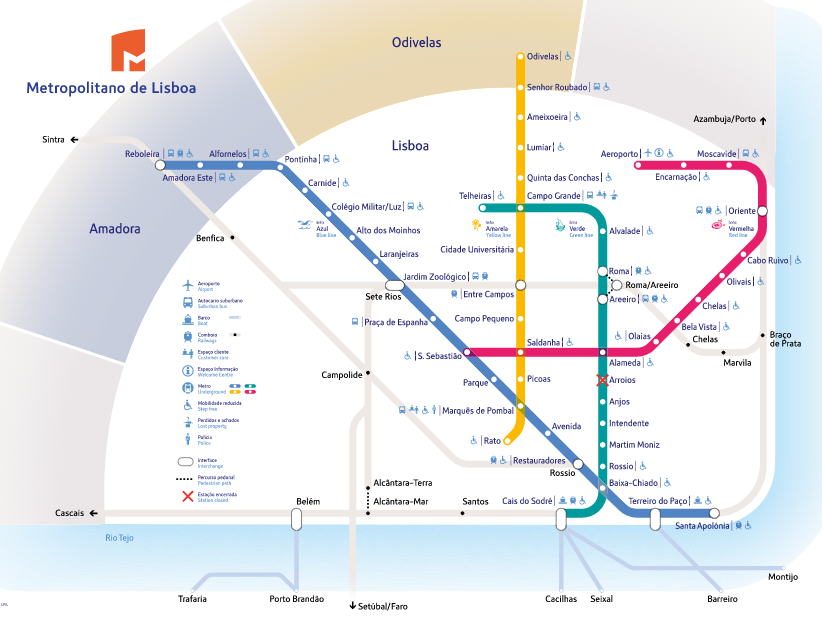
\includegraphics[scale=0.3]{metro.png}
	\end{center}

\end{frame}

\begin{frame}
	\frametitle{Modelos em Economia}
	\begin{itemize}
		\item S\~ao uma forma de ultrapassar a complexidad da realidad e evitar que se cometam erros de an\'alise - abordagem \emph{c\ae teris paribus} \pause
		\item S\~ao instrumentos de an\'alise que permitem sintetizar ideias e analisar problemas de forma objectiva e condensada.\pause
		\item Tal como um mapa de estradas, um modelo n\~ao \'e um retrato da realidade, mas \'e uma representa\c c\~ao simplificada que permite tirar conclus\~oes acerca de como funciona a realidade.
	\end{itemize}

\end{frame}

\begin{frame}
	\frametitle{Um modelo...}
	\begin{itemize}
		\item Permite conclus\~oes v\'alidas, sem cair em erros de dedu\c c\~ao;\pause
		\item baseia-se em pressupostos/hip\'oteses;\pause
		\item explicita e precisa, simplificando a realidade;\pause
		\item recorre a equa\c c\~oes e gr\'aficos para descrever as rela\c c\~oes entre os factores que est\~ao a ser estudados.
		\end{itemize}
\end{frame}

\begin{frame}
	\frametitle{Esquema geral do modelo Micro}
	\begin{center}	
		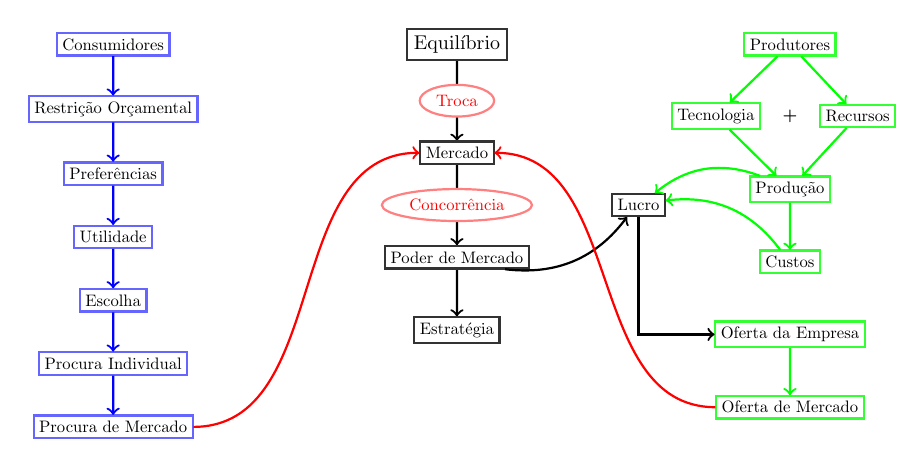
\begin{tikzpicture}[thick,scale=0.5, every node/.style={scale=0.6}]
			\onslide<3->{	
				\node[rectangle, draw=black!80, scale = 1.2] (eq) {Equil\'ibrio};
				\node[ellipse, red, draw = red!50, fill=white!80 , below = 3mm of eq] (troca) {Troca};
				\node[rectangle, draw=black!80, below = 3mm of troca] (mkt) {Mercado};\
				\node[ellipse, red, draw = red!50, fill=white!80 , below = 3mm of mkt] (comp) {Concorr\^encia};
				\node[rectangle, draw=black!80, below = 3mm  of comp] (mktpow) {Poder de Mercado};
				\node[rectangle, draw=black!80, below = 6mm of mktpow] (strat) {Estrat\'egia};
			}
			\onslide<2->{
				\node[rectangle, draw=black!80, right = of comp] (profit) {Lucro};
			}

			\onslide<1->{
				\node[rectangle, draw=blue!60, left = 30mm of eq] (cons) {Consumidores};
				\node[rectangle, draw=blue!60, below = 5mm of cons] (bc) {Restri\c c\~ao Or\c camental};
				\node[rectangle, draw=blue!60, below = 5mm of bc] (pref) {Prefer\^encias};
				\node[rectangle, draw=blue!60, below = 5mm of pref] (ut) {Utilidade};
				\node[rectangle, draw=blue!60, below = 5mm of ut] (ch) {Escolha};
				\node[rectangle, draw=blue!60, below = 5mm of ch] (id) {Procura Individual};
				\node[rectangle, draw=blue!60, below = 5mm of id] (md) {Procura de Mercado};
			}

			\onslide<2->{
				\node[rectangle, draw=green!80, right = 30mm of eq] (firm) {Produtores};
				\node[below = 6mm of firm] (plus) {\textbf{+}};
				\node[rectangle, draw=green!80, left = 2mm of plus] (tec) {Tecnologia};
				\node[rectangle, draw=green!80, right = 2mm of plus] (res) {Recursos};
				\node[rectangle, draw=green!80, below = 6mm of plus] (prod) {Produ\c c\~ao};
				\node[rectangle, draw=green!80, below = 6mm of prod] (costs) {Custos};
				\node[rectangle, draw=green!80, below = 6mm of costs] (fsup) {Oferta da Empresa};
				\node[rectangle, draw=green!80, below = 6mm of fsup] (msup) {Oferta de Mercado};
			}

			\onslide<3->{
				\draw[thick,->]	(mktpow) edge [bend right] (profit);
			}
			\onslide<2->{
				\draw[green,thick,->] (prod) edge [bend right]  (profit);
				\draw[green,thick,->] (costs) edge [bend right] (profit);
				\draw[thick,->] (profit) |- (fsup);
			}

			\onslide<1->{
				\draw[thick,blue,->]	(cons) -- (bc);
				\draw[thick,blue,->]	(bc) -- (pref);
				\draw[thick,blue,->]	(pref) -- (ut);
				\draw[thick,blue,->]	(ut) -- (ch);
				\draw[thick,blue,->]	(ch) -- (id);
				\draw[thick,blue,->]	(id) -- (md);
			}

			\onslide<3->{
				\draw[->,red,thick] (md) to [out=0,in=180] (mkt);
				\draw[->,red,thick] (msup) to [out=180,in=0] (mkt);
			}

			\onslide<2->{
				\draw[thick,green,->] (firm) -- (tec);
				\draw[thick,green,->] (firm) -- (res);
				\draw[thick,green,->] (tec) -- (prod);
				\draw[thick,green,->] (res) -- (prod);
				\draw[thick,green,->] (prod) -- (costs);
				\draw[thick,green,->] (fsup) -- (msup);
			}

			\begin{pgfonlayer}{bg}
				\onslide<3->{
					\draw[thick,->] (eq) -- (mkt);
					\draw[thick,->] (mkt) -- (mktpow);
					\draw[thick,->] (mktpow) -- (strat);
				}
			\end{pgfonlayer}

		\end{tikzpicture}
	\end{center}

\end{frame}

\begin{frame}
	\frametitle{A Fronteira das Possibilidades de Produ\c c\~ao}

	Descreve a produ\c c\~ao m\'axima que \'e poss\'ivel obter, para um conjunto de bens, dados os recursos dispon\'iveis numa economia.

	\vspace{0.2cm}

	No modelo:\pause
	\begin{itemize}
		\item consideram-se dois bens; \pause
		\item admite-se que a tecnologia e os recursos s\~ao fixos; \pause
		\item ilustra-se o conceito de efici\^encia de Pareto; \pause
		\item utiliza-se o conceito de custo de oportunidade;
	\end{itemize}

\end{frame}

\begin{frame}
	\frametitle{Fronteira das Possibilidades de Produ\c c\~ao}

	\begin{columns}
		\begin{column}{0.47\textwidth}
			\begin{center}
				\begin{tikzpicture}[scale=0.7,every node/.style={scale=0.7}]
					\draw[->] (-0.1,0) -- (4,0) node[below right] {Bem $X$};
					\draw[->] (0,-0.1) -- (0,4) node[above left] {Bem $Y$};

					\draw[] (0,2) node[left] {$A$} -- (3,0) node[below] {$B$};

					\node[circle,fill=black,inner sep=0pt,minimum size=3pt,label=left:{$M$}] at (.8,.8) {};
					\node[circle,fill=black,inner sep=0pt,minimum size=3pt,label=left:{$N$}] at (2,2) {};
				\end{tikzpicture}
			\end{center}
			$M$: Ineficiente, \quad $N$: inating\'ivel
		\end{column}
		\begin{column}{0.47\textwidth}
			\scriptsize{
			\begin{itemize}
				\item Os pontos A e B representam produ\c c\~ao com especializa\c c\~ao em cada uma das actividades \pause
				\item Pontos sobre a FPP s\~ao pontos de produ\c c\~ao eficientes no sentido de Pareto \pause
				\item A partir de um ponto da FPP, caso se queira aumentar a produ\c c\~ao de um bem, \'e preciso prescindir da produ\c c\~ao de outro na raz\~ao $\left|\frac{\Delta Y}{\Delta X}\right|$.\pause
				\item $\left|\frac{\Delta Y}{\Delta X}\right|$ coincide com o declive da FPP linear (sem sinal) e designa-se custo relativo do bem $X$. Representa um \emph{custo de oportunidade}...
			\end{itemize}
			}
		\end{column}
	\end{columns}
\end{frame}

\begin{frame}
	\frametitle{Fronteira das Possibilidades de Produ\c c\~ao}
	\begin{columns}
		\begin{column}{0.47\textwidth}
			\begin{center}
				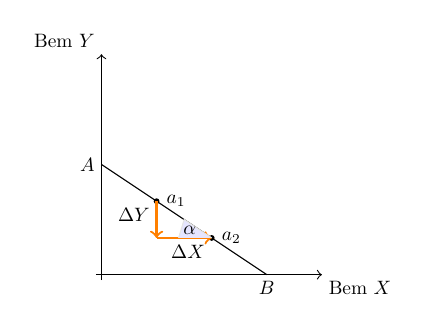
\begin{tikzpicture}[scale=0.7,every node/.style={scale=0.7}]
					\draw[->] (-0.1,0) -- (4,0) node[below right] {Bem $X$};
					\draw[->] (0,-0.1) -- (0,4) node[above left] {Bem $Y$};

					\draw[] (0,2) node[left] {$A$} -- (3,0) node[below] {$B$};

					\node[circle,fill=black,inner sep=0pt,minimum size=3pt,label=right:{$a_1$}] at (1,{4/3}) {};
					\node[circle,fill=black,inner sep=0pt,minimum size=3pt,label=right:{$a_2$}] at (2,{2/3}) {};

					\onslide<2->{
						\draw[orange,->,thick] (1,{4/3}) -- (1,{2/3});
						\node[below left] at (1,{4/3}) {$\Delta Y$};
					}

					\onslide<3->{
						\draw[orange,->,thick] (1,{2/3}) -- (2,{2/3});
						\node[below left] at (2,{2/3}) {$\Delta X$};
					}

					\onslide<4->{
						\draw[draw=black!10,fill=blue!10] (2,{2/3}) -- (1.5,1) -- (1.4,{2/3}); 
						\node[] at (1.6,.8) {$\alpha$};
					}

				\end{tikzpicture}
			\end{center}
		\end{column}
		
		\begin{column}{0.47\textwidth}
			\begin{itemize}
				\item \onslide<5->{$\left|\frac{\Delta Y}{\Delta X}\right|=|\tan{\alpha}|$, o que coincide com o declive da FPP linear (sem sinal) e designa-se custo relativo do bem $X$.}
				\item \onslide<6->{Representa um custo de oportunidade...}
			\end{itemize}
		\end{column}
	\end{columns}

\end{frame}

\begin{frame}
	\frametitle{Vantagens do Com\'ercio}

	\begin{itemize}
		\item H\'a ganhos que decorrem de os indiv\'iduos se especializarem nas tarefas que fazem melhor e recorrerem ao com\'ercio para trocarem entre si o produto das suas actividades \pause
		\item Usemos a FPP para tirar essa conclus\~ao
	\end{itemize}
\end{frame}

\begin{frame}
	\frametitle{Vantagens do Com\'ercio}
	Dois vizinhos, um sabe pintar e o outro sabe cozinhar... as suas FPP s\~ao descritas por:

	\vspace{0.1cm}

	\begin{columns}
		\begin{column}{0.47\textwidth}
			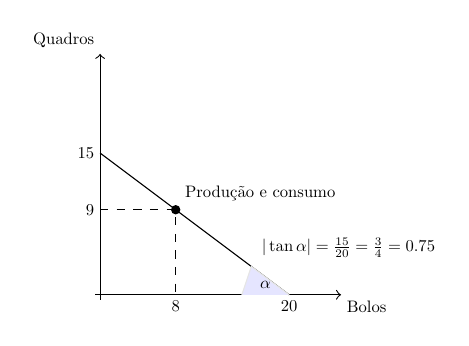
\begin{tikzpicture}[scale = 0.6, every node/.style={scale=0.6}]
				\draw[->] (-0.1,0) -- (5.1,0) node[below right] {Bolos};
				\draw[->] (0,-0.1) -- (0,5.1) node[above left] {Quadros};

				\draw[black] (0,3) node[left] {$15$} -- (4,0) node[below]{$20$};
				\draw[dashed] (0,1.8) node[left] {$9$} -- (1.6,1.8) node[circle,fill,inner sep=2pt,label=above right:Produ\c c\~ao e consumo]{} -- (1.6,0) node[below]{$8$};

				\draw[draw=black!10,fill=blue!10] (4,0) -- (3.2,.6) -- (3,0); 
				\node[] at (3.5,.2) {$\alpha$};

				\node[anchor = west] at (3.3,1) {$|\tan{\alpha}|=\frac{15}{20}=\frac{3}{4}=0.75$};
			\end{tikzpicture}
			\centering{\small{Pintor}}
		\end{column}
		\begin{column}{0.47\textwidth}
			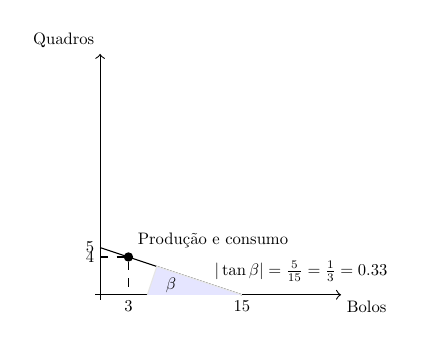
\begin{tikzpicture}[scale = 0.6, every node/.style={scale=0.6}]
				\draw[->] (-0.1,0) -- (5.1,0) node[below right] {Bolos};
				\draw[->] (0,-0.1) -- (0,5.1) node[above left] {Quadros};

				\draw[black] (0,1) node[left] {$5$} -- (3,0) node[below]{$15$};
				\draw[dashed] (0,0.8) node[left] {$4$} -- (0.6,0.8) node[circle,fill,inner sep=2pt,label=above right:Produ\c c\~ao e consumo]{} -- (0.6,0) node[below]{$3$};

				\draw[draw=black!10,fill=blue!10] (3,0) -- (1.2,.6) -- (1,0); 
				\node[] at (1.5,.2) {$\beta$};

				\node[anchor = west] at (2.3,0.5) {$|\tan{\beta}|=\frac{5}{15}=\frac{1}{3}=0.33$};
			\end{tikzpicture}
			\centering{\small{Cozinheiro}}
		\end{column}
	\end{columns}
\end{frame}

\begin{frame}
	\frametitle{Custos Relativos; Vantagem Comparativa}

	\begin{table}
		{\renewcommand{\arraystretch}{1.5}
		\begin{tabular}{cccc}
			Custos de Oportunidade & Pintor & & Cozinheiro \\
			\hline \hline
			Um bolo & $\frac{3}{4}$ & $>$ & $\frac{1}{3}$ \\
			Um quadro & $\frac{4}{3}$ & $<$ & $3$ \\
			\hline \hline
		\end{tabular}
		}
	\end{table}\pause
	\small{
	O cozinheiro tem vantagem comparativa na produ\c c\~ao de bolos, no entanto o pintor tem vantagem comparativa na produ\c c\~ao de quadros... \pause

	\vspace{0.2cm}

	Valer\'a a pena o pintor especializar-se na produ\c c\~ao de quadros se puder trocar cada um por mais do que $\frac{4}{3}$ de bolos (o custo de oportunidade)\pause

	\vspace{0.2cm}

	Valer\'a a pena o cozinheiro especializar-se na produ\c c\~ao de bolos, se puder trocar cada um por mais do que $\frac{1}{3}$ de quadro (ou seja, um quadro em troca de $3$ bolos no m\'aximo)	
	}
\end{frame}

\begin{frame}
	\frametitle{Termos de Troca}

	Estando o pintor disposto a receber $\frac{4}{3}$ de bolo por cada quadro que venda e estando o cozinheiro disposto a pagar $3$ bolos por cada quadro que compre, h\'a margem para transac\c c\~oes mutuamente vantajosas! \pause

	\vspace{0.2cm}

	Pode haver trocas se um quadro se trocar por um qualquer n\'umero de bolos entre $\frac{4}{3}$ e $3$.

\end{frame}

\begin{frame}
	\frametitle{Vantagens do com\'ercio}
	{\small Admitamos que h\'a especializa\c c\~ao e que o pintor vende $5$ quadros ao cozinheiro e que lhe compra $10$ bolos em troca... ent\~ao cada quadro trasaccionou-se em troca de $2$ bolos, o que \'e um valor interm\'edio entre o valor que o pintor estava disposto a receber para vender um quadro e o valor que o cozinheiro estava disposto a pagar.}
	
	\begin{table}
		\begin{adjustbox}{max width = \textwidth}
		{\renewcommand{\arraystretch}{1.5}
		\begin{tabular}{ccccccc}
			\multicolumn{2}{c}{} & \multicolumn{2}{c}{Autarcia} & \multicolumn{2}{c}{Com Com\'ercio} & \multirow{2}{*}{\parbox{2cm}{Ganhos de com\'ercio}}\\
			\cline{3-4}\cline{5-6} 
			\multicolumn{2}{c}{} & Produ\c c\~ao & Consumo & Produ\c c\~ao & Consumo & \\
			\hline\hline
			\multirow{2}{*}{Pintor} & Quadros & 9 & 9 & 15 & 10 & +1 \\
								    & Bolos   & 8 & 8 & 0  & 10 & +2 \\
			\hline
			\multirow{2}{*}{Cozinheiro} & Quadros & 4 & 4 & 0 & 5 & +1 \\
										& Bolos & 3 & 3 & 15 & 5 & +2 \\
			\hline\hline
		\end{tabular}
		}
		\end{adjustbox}
	\end{table}
\end{frame}

\begin{frame}
	\frametitle{Vantagens do Com\'ercio}
	Com com\'ercio, ambos os agentes econ\'omicos beneficiam, \\
	especializando-se no que fazem melhor (vantagem comparativa)

	\vspace{0.1cm}

	\begin{columns}
		\begin{column}{0.47\textwidth}
			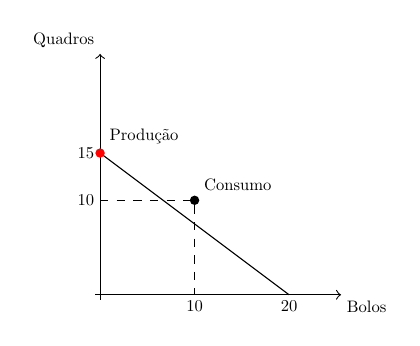
\begin{tikzpicture}[scale = 0.6, every node/.style={scale=0.6}]
				\draw[->] (-0.1,0) -- (5.1,0) node[below right] {Bolos};
				\draw[->] (0,-0.1) -- (0,5.1) node[above left] {Quadros};

				\draw[black] (0,3) node[left] {$15$} -- (4,0) node[below]{$20$};
				\draw[dashed] (0,2) node[left] {$10$} -- (2,2) node[circle,fill,inner sep=2pt,label=above right:Consumo]{} -- (2,0) node[below]{$10$};

				\draw (0,3) node[red,circle,fill,inner sep=2pt,label=above right:Produ\c c\~ao]{};
			\end{tikzpicture}
			\centering{\small{Pintor}}
		\end{column}
		\begin{column}{0.47\textwidth}
			\begin{tikzpicture}[scale = 0.6, every node/.style={scale=0.6}]
				\draw[->] (-0.1,0) -- (5.1,0) node[below right] {Bolos};
				\draw[->] (0,-0.1) -- (0,5.1) node[above left] {Quadros};

				\draw[black] (0,1) node[left] {$5$} -- (3,0) node[below]{$15$};
				\draw[dashed] (0,1) node[left] {$5$} -- (1,1) node[circle,fill,inner sep=2pt,label=above right:Consumo]{} -- (1,0) node[below]{$5$};

				\draw (3,0) node[red,circle,fill,inner sep=2pt,label=above right:Produ\c c\~ao]{};

			\end{tikzpicture}
			\centering{\small{Cozinheiro}}
		\end{column}
	\end{columns}
\end{frame}

\begin{frame}
	\frametitle{Vantagens do Com\'ercio}
	Possibilidades de Consumo se termos de troca forem 1 quadro trocado por 2 bolos...

	\vspace{0.1cm}

	\begin{columns}
		\begin{column}{0.47\textwidth}
			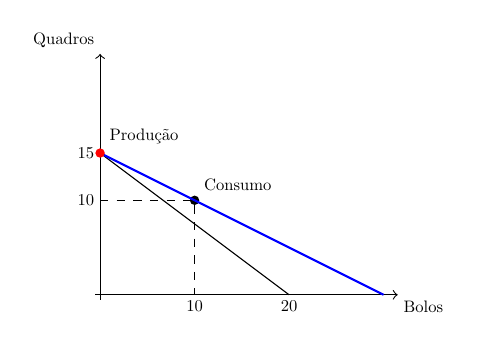
\begin{tikzpicture}[scale = 0.6, every node/.style={scale=0.6}]
				\draw[->] (-0.1,0) -- (6.3,0) node[below right] {Bolos};
				\draw[->] (0,-0.1) -- (0,5.1) node[above left] {Quadros};

				\draw[black] (0,3) node[left] {$15$} -- (4,0) node[below]{$20$};
				\draw[dashed] (0,2) node[left] {$10$} -- (2,2) node[circle,fill,inner sep=2pt,label=above right:Consumo]{} -- (2,0) node[below]{$10$};

				\draw[blue, thick] (0,3) -- (6,0);

				\draw (0,3) node[red,circle,fill,inner sep=2pt,label=above right:Produ\c c\~ao]{};
			\end{tikzpicture}
			\centering{\small{Pintor}}
		\end{column}
		\begin{column}{0.47\textwidth}
			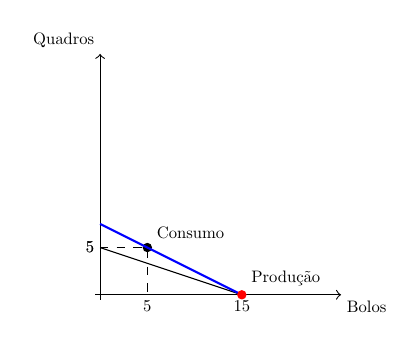
\begin{tikzpicture}[scale = 0.6, every node/.style={scale=0.6}]
				\draw[->] (-0.1,0) -- (5.1,0) node[below right] {Bolos};
				\draw[->] (0,-0.1) -- (0,5.1) node[above left] {Quadros};

				\draw[black] (0,1) node[left] {$5$} -- (3,0) node[below]{$15$};
				\draw[dashed] (0,1) node[left] {$5$} -- (1,1) node[circle,fill,inner sep=2pt,label=above right:Consumo]{} -- (1,0) node[below]{$5$};

				\draw[blue,thick] (0,1.5) -- (3,0);

				\draw (3,0) node[red,circle,fill,inner sep=2pt,label=above right:Produ\c c\~ao]{};

			\end{tikzpicture}
			\centering{\small{Cozinheiro}}
		\end{column}
	\end{columns}
\end{frame}

\begin{frame}
	\frametitle{Vantagem comparativa}
	\begin{itemize}
		\item No exemplo, o pintor tem vantagem comparativa na produ\c c\~ao de quadros porque o seu custo de oportunidade \'e menor do que o do cozinheiro: precisa de prescindir de menor quantidade de produ\c c\~ao de bolos para utilizar o seu tempo na produ\c c\~ao de quadros do que o cozinheiro precisaria se quisesse produzir mais um quadro...

		\item \'E da vantagem comparativa que dependem os ganhos do com\'ercio e os padr\~oes de especializa\c c\~ao
	\end{itemize}
\end{frame}

\begin{frame}
	\frametitle{Vantagem comparativa}
	\begin{itemize}
		\item O com\'ercio (neste caso, troca directa) tem a vantagem de permitir que cada um dos agentes econ\'omicos se especialize na tarfe que faz relativemnte melhor, para que depois eles se encontrem no mercado para fazerem transac\c c\~oes.
		\item Ap\'os o com\'ercio, \'e poss\'ivel os indiv\'iduos estarem num ponto de consumo em que obt\^em mais quantidade de ambos os bens, do que numa situa\c c\~ao de autarcia, usando so mesmos recursos.

		\item Todos temos uma vantagem comparativa nalguna actividade... o mesmo se aplica a empresas, a pa\'ises... \'e neste princ\'ipio que se baseia o com\'ercio internacional.
	\end{itemize}
\end{frame}
\section{FPP - Modelos n\~ao lineares}
\begin{frame}
	\frametitle{Fronteira das Possibilidades de Produ\c c\~ao}

	\begin{columns}
		\begin{column}{0.47\textwidth}
			\scriptsize{
			\begin{tabular}{ccc}
				\multirow{2}{*}{\parbox{2cm}{Possibilidades de Produ\c c\~ao}} & \multirow{2}{*}{Bem $X$} & \multirow{2}{*}{Bem $Y$} \\
				 & & \\
				 \hline \hline
				 A & 0 & 30 \\
				 B & 2 & 28 \\
				 C & 4 & 24 \\
				 D & 6 & 18 \\
				 E & 8 & 10 \\
				 F & 10 & 0 \\
				 \hline\hline 				
			\end{tabular}
			}
		\end{column}
		\begin{column}{0.47\textwidth}
			\begin{center}
				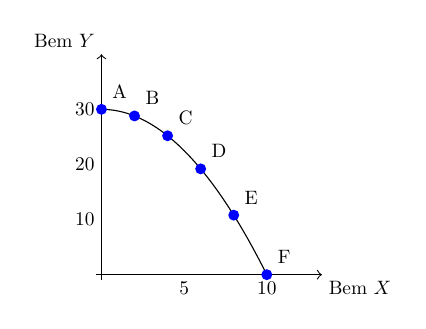
\begin{tikzpicture}[
					scale=0.7,
					every node/.style={scale=0.7},
					declare function = {fpp(\x) = 3 - (1/3) * \x^(2);}
					]

					\draw[->] (-0.1,0) -- (4,0) node[below right] {Bem $X$};
					\draw[->] (0,-0.1) -- (0,4) node[above left] {Bem $Y$};

					\draw[smooth,domain=0:3,variable=\x] plot (\x,{fpp(\x)});

					\draw (0,{fpp(0)}) node[blue,circle,fill,inner sep=2pt,label=above right:A]{};
					\draw (0.6,{fpp(0.6)}) node[blue,circle,fill,inner sep=2pt,label=above right:B]{};
					\draw (1.2,{fpp(1.2)}) node[blue,circle,fill,inner sep=2pt,label=above right:C]{};
					\draw (1.8,{fpp(1.8)}) node[blue,circle,fill,inner sep=2pt,label=above right:D]{};
					\draw (2.4,{fpp(2.4)}) node[blue,circle,fill,inner sep=2pt,label=above right:E]{};
					\draw (3,{fpp(3)}) node[blue,circle,fill,inner sep=2pt,label=above right:F]{};

					\draw (0,3) node[left] {30};
					\draw (0,2) node[left] {20};
					\draw (0,1) node[left] {10};

					\draw(1.5,0) node[below] {5};
					\draw(3,0) node[below] {10};

				\end{tikzpicture}
			\end{center}
		\end{column}
	\end{columns}
\end{frame}

\begin{frame}
	\frametitle{Custo relativo}
	$$CO_X = TMT_{Y,X}=-\frac{\Delta Y}{\Delta X}$$
	\begin{center}
		\begin{tabular}{cccc}
			Possibilidade de produ\c c\~ao & Bem $X$ & Bem $Y$ & $TMT_{Y,X}$ \\
			\hline\hline
			A & 0 & 30 & - \\
			B & 2 & 28 & 1 \\
			C & 4 & 24 & 2 \\
			D & 6 & 18 & 3 \\
			E & 8 & 10 & 4 \\
			F & 10 & 0 & 5 \\
			\hline \hline
		\end{tabular}
	\end{center}
\end{frame}

\begin{frame}
	\frametitle{Custo Relativo Crescente}
	\begin{center}
		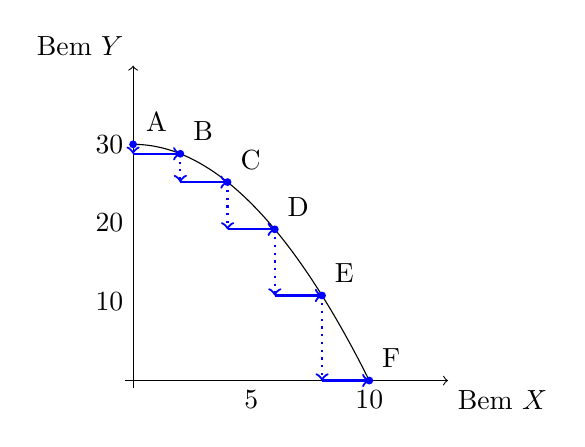
\begin{tikzpicture}[
			scale=1,
			every node/.style={scale=1},
			declare function = {fpp(\x) = 3 - (1/3) * \x^(2);}
			]

			\draw[->] (-0.1,0) -- (4,0) node[below right] {Bem $X$};
			\draw[->] (0,-0.1) -- (0,4) node[above left] {Bem $Y$};

			\draw[smooth,domain=0:3,variable=\x] plot (\x,{fpp(\x)});

			\draw (0,{fpp(0)}) node[blue,circle,fill,inner sep=1pt,label=above right:A]{};
			\draw (0.6,{fpp(0.6)}) node[blue,circle,fill,inner sep=1pt,label=above right:B]{};
			\draw (1.2,{fpp(1.2)}) node[blue,circle,fill,inner sep=1pt,label=above right:C]{};
			\draw (1.8,{fpp(1.8)}) node[blue,circle,fill,inner sep=1pt,label=above right:D]{};
			\draw (2.4,{fpp(2.4)}) node[blue,circle,fill,inner sep=1pt,label=above right:E]{};
			\draw (3,{fpp(3)}) node[blue,circle,fill,inner sep=1pt,label=above right:F]{};

			\draw (0,3) node[left] {30};
			\draw (0,2) node[left] {20};
			\draw (0,1) node[left] {10};

			\draw(1.5,0) node[below] {5};
			\draw(3,0) node[below] {10};

			\foreach \x in {0,...,4}
				{
				\draw[blue,thick,dotted,->] ({\x*0.6},{fpp((\x*0.6))}) -- ({\x*0.6},{fpp((\x*0.6+0.6))});
				\draw[blue,thick,->] ({\x*0.6},{fpp((\x*0.6+0.6))}) -- ({(\x*0.6+0.6)},{fpp((\x*0.6+0.6))});
				}	

		\end{tikzpicture}
	\end{center}

\end{frame}

\begin{frame}
	\frametitle{Custo Relativo - Derivada da FPP}
	\begin{columns}
		\begin{column}{0.47\textwidth}
			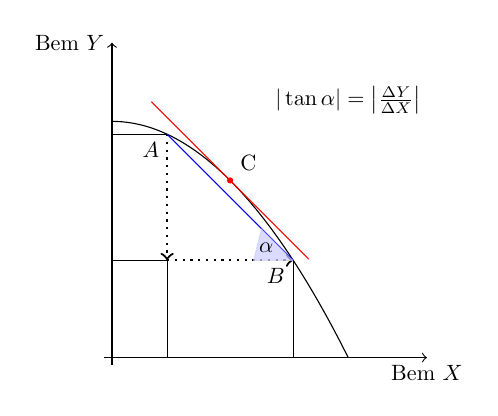
\begin{tikzpicture}[
			scale=1,
			every node/.style={scale=0.8},
			declare function = {fpp(\x) = 3 - (1/3) * \x^(2);},
			declare function = {tfpp(\x) = (15/4) - \x;}
			]
			\def\a{0.7}
			\def\b{2.3}
			\def\d{1.5}

			\draw[->] (-0.1,0) -- (4,0) node[below] {Bem $X$};
			\draw[->] (0,-0.1) -- (0,4) node[left] {Bem $Y$};

			\draw[smooth,domain=0:3,variable=\x] plot (\x,{fpp(\x)});

			\draw (3,3) node[above] {$|\tan \alpha|=\left|\frac{\Delta Y}{\Delta X}\right|$};

			\draw (0,{fpp(\a)}) -- (\a,{fpp(\a)}) node[below left] {$A$};
			\draw (0,{fpp(\b)}) -- (\a,{fpp(\b)});
			\draw[dotted,thick,->] (\a,{fpp(\a)}) -- (\a,{fpp(\b)});
			\draw[dotted,thick,->] (\a,{fpp(\b)}) -- (\b,{fpp(\b)})node[below left] {$B$};
			\draw (\a,{fpp(\b)}) -- (\a,0);
			\draw (\b,{fpp(\b)}) -- (\b,0);

			\draw[blue] (\a,{fpp(\a)}) -- (\b,{fpp(\b)});

			\draw[red,domain=0.5:2.5,variable=\x] plot (\x,{tfpp(\x)});
			\draw (\d,{fpp(\d)}) node[red,circle,fill,inner sep=1pt,label=above right:C]{};

			\draw[fill,blue!20,opacity=0.7] (\b,{fpp(\b)}) -- ({(\b-0.5)},{fpp(\b)}) -- ({\b-0.4},{fpp(\b)+0.4});
			\draw (\b-0.15,{fpp(\b)}) node[above left] {$\alpha$};

			\end{tikzpicture}
		\end{column}
		\begin{column}{0.47\textwidth}
			{\scriptsize
			\begin{itemize}
				\item $\frac{\Delta Y}{\Delta X}$ \'e a taxa de varia\c c\~ao m\'edia: qual a varia\c c\~ao em $Y$ por unidade de varia\c c\~ao em $X$...
				\item $\left|\frac{\Delta Y}{\Delta X}\right|$ \'e o custo relativo de uma unidade adicional de $X$
				\item $\left|\frac{\Delta Y}{\Delta X}\right|$ \'e o custo de oportunidade de uma unidade adicional de $X$
				\item $\frac{\Delta Y}{\Delta X}$ \'e o declive da recta tangente no ponto $C$ (Lagrange)... \'e a derivada \`a FPP nesse ponto
			\end{itemize}
			}
		\end{column}
	\end{columns}
\end{frame}

\begin{frame}
	\frametitle{Vantagens do Com\'ercio}
	Vamos admitir que podemos aceder a um mercado onde podemos transacionar $y$ unidades do bem $Y$ por $x$ unidades do bem $X$. O que temos ent\~ao \'e algo similar ao que t\'inhamos na aula anterior, termos de troca constantes, mas a nossa FPP n\~ao mudou.
	\begin{center}
		\begin{tikzpicture}[
				scale=1,
				every node/.style={scale=0.8},
				declare function = {fpp(\x) = 3 - (1/3) * \x^(2);},
				declare function = {mkt1(\x) = 3 - 0.8*\x;},
				declare function = {mkt2(\x) = 4 - 0.8*\x;},
				declare function = {mkt3(\x) = 3.5 - 0.8*\x;}
				]

				\draw[->] (-0.1,0) -- (5.2,0) node[below] {Bem $X$};
				\draw[->] (0,-0.1) -- (0,5) node[left] {Bem $Y$};

				\draw[smooth,domain=0:3,variable=\x] plot (\x,{fpp(\x)});
				\draw (0,{fpp(0)}) node[left] {$Y_0$};
				\draw (3,{fpp(3)})node[below] {$X_0$};
				
				\only<2>{
					\draw[red,domain=0:(3/0.8),variable=\x] plot (\x,{mkt1(\x)});
				}

				\only<3>{
					\draw[red,dashed,domain=0:2.45,variable=\x] plot (\x,{mkt1(\x)});
					\draw[red,domain=2.45:(3/0.8),variable=\x] plot (\x,{mkt1(\x)});
				}

				\only<4>{
					\draw[red,domain=0:(4/0.8),variable=\x] plot (\x,{mkt2(\x)});
				}

				\only<5>{
					\draw[red,domain=0:(3.5/0.8),variable=\x] plot (\x,{mkt3(\x)});
				}


		\end{tikzpicture}
	\end{center}
\end{frame}

\begin{frame}
	\frametitle{Vantagens do Com\'ercio}
	\begin{columns}
		\begin{column}{0.47\textwidth}
			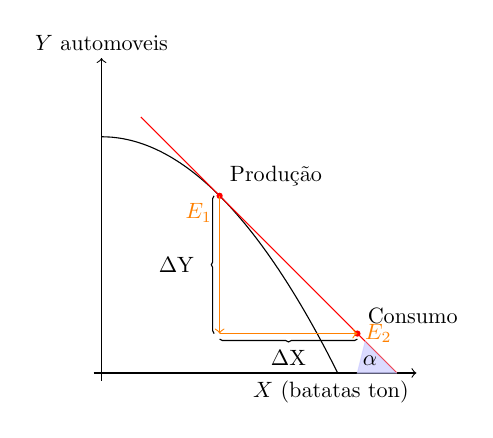
\begin{tikzpicture}[
			scale=1,
			every node/.style={scale=0.8},
			declare function = {fpp(\x) = 3 - (1/3) * \x^(2);},
			declare function = {tfpp(\x) = (15/4) - \x;}
			]

			\def\d{1.5}
			\def\e{3.25}

			\draw[->] (-0.1,0) -- (4,0) node[below left] {$X$ (batatas ton)};
			\draw[->] (0,-0.1) -- (0,4) node[above] {$Y$ automoveis};

			\draw[smooth,domain=0:3,variable=\x] plot (\x,{fpp(\x)});

			\draw[red,domain=0.5:(15/4),variable=\x] plot (\x,{tfpp(\x)});
			\draw (\d,{fpp(\d)}) node[red,circle,fill,inner sep=1pt,label=above right:Produ\c c\~ao]{};
			\draw (\e,{tfpp(\e)}) node[red,circle,fill,inner sep=1pt,label=above right:Consumo]{};

			\draw[orange,->] (\d,{fpp(\d)}) node[below left] {$E_1$} -- (\d,{tfpp(\e)});
			\draw[orange,->] (\d,{tfpp(\e)}) -- (\e,{tfpp(\e)}) node[right] {$E_2$};

			\draw[fill,blue!20,opacity=0.7] ({(15/4)},{tfpp((15/4))}) -- ({(15/4)-0.5},{tfpp((15/4))}) -- ({(15/4)-0.4},{tfpp((15/4))+0.4});
			\draw ({(15/4)-0.15},{tfpp((15/4))}) node[above left] {$\alpha$};

			\draw [decorate,decoration={brace,amplitude=1pt},xshift=-2pt,yshift=0pt] (\d,{tfpp(\e)}) -- (\d,{tfpp(\d)}) node [black,midway,xshift=-0.6cm] {$\Delta$Y};
			\draw [decorate,decoration={brace,mirror,amplitude=1pt},xshift=0pt,yshift=-2pt] (\d,{tfpp(\e)}) -- (\e,{tfpp(\e)}) node [black,midway,yshift=-0.3cm] {$\Delta$X};

			\end{tikzpicture}
			$\Delta Y$: Exporta\c c\~ao\\
			$\Delta X$: Importa\c c\~ao
		\end{column}
		\begin{column}{0.47\textwidth}
			{\scriptsize
			\begin{itemize}
				\item 1 autom\'ovel vende-se internacionalmente por $p_y=\textup{\euro}8,000$
				\item 1 ton de batatas vende-se internacionalmente por $p_x=\textup{\euro}1,000$
				\item Termos de troca: 1 autom\'ovel troca-se por 8 ton de batata $\frac{p_x}{p_y}=\frac{1}{8}$
				\item A fronteira de possibilidades de consumo ter\'a declive $\frac{1}{8}$ a partir do ponto de produ\c c\~ao $E_1$.
				\item Se o consumo for em $E_2$, esta economia exporta automoveis para importar batatas e verifica-se que:$$\Delta Y p_y + \Delta X p_x = 0$$
			\end{itemize}
			}
		\end{column}
	\end{columns}
\end{frame}

\begin{frame}
	\frametitle{Vantagens do Com\'ercio}
	\begin{columns}
		\begin{column}{0.47\textwidth}
			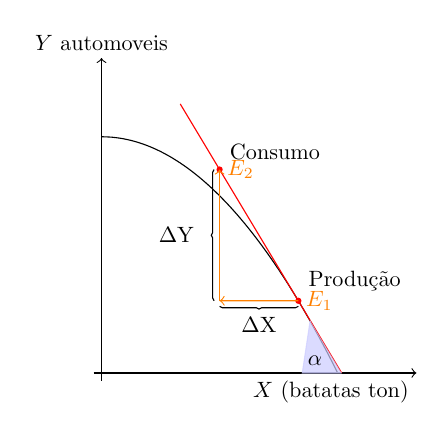
\begin{tikzpicture}[
			scale=1,
			every node/.style={scale=0.8},
			declare function = {fpp(\x) = 3 - (1/3) * \x^(2);},
			declare function = {tfpp(\x) = (61/12) - (5/3)*\x;}
			]

			\def\d{2.5}
			\def\e{1.5}

			\draw[->] (-0.1,0) -- (4,0) node[below left] {$X$ (batatas ton)};
			\draw[->] (0,-0.1) -- (0,4) node[above] {$Y$ automoveis};

			\draw[smooth,domain=0:3,variable=\x] plot (\x,{fpp(\x)});
			\draw[red,domain=1:3.05,variable=\x] plot (\x,{tfpp(\x)});

			\draw (\d,{fpp(\d)}) node[red,circle,fill,inner sep=1pt,label=above right:Produ\c c\~ao]{};
			\draw (\e,{tfpp(\e)}) node[red,circle,fill,inner sep=1pt,label=above right:Consumo]{};

			\draw[orange,->] (\d,{fpp(\d)}) node[right] {$E_1$} -- (\e,{tfpp(\d)});
			\draw[orange,->] (\e,{tfpp(\d)}) -- (\e,{tfpp(\e)}) node[right] {$E_2$};

			\draw[fill,blue!20,opacity=0.7] (3.05,{tfpp((3.05))}) -- ({3.05-0.5},{tfpp(3.05)}) -- ({3.05-0.4},{tfpp(3.05-0.4)});
			\draw ({3-0.1},{tfpp(3.05)}) node[above left] {$\alpha$};

			\draw [decorate,decoration={brace,amplitude=1pt},xshift=-2pt,yshift=0pt] (\e,{tfpp(\d)}) -- (\e,{tfpp(\e)}) node [black,midway,xshift=-0.6cm] {$\Delta$Y};
			\draw [decorate,decoration={brace,mirror,amplitude=1pt},xshift=0pt,yshift=-2pt] (\e,{tfpp(\d)}) -- (\d,{tfpp(\d)}) node [black,midway,yshift=-0.3cm] {$\Delta$X};

			\end{tikzpicture}
			$\Delta Y$: Importa\c c\~ao\\
			$\Delta X$: Exporta\c c\~ao
		\end{column}
		\begin{column}{0.47\textwidth}
			{\scriptsize
			\begin{itemize}
				\item Uma unidade de $Y$ vende-se internacionalmente por $p_y$
				\item Uma unidade de $X$ vende-se internacionalmente por $p_x$
				\item Termos de troca: 1 unidade de $X$ troca-se por $\frac{p_x}{p_y}$ unidades de $Y$
				\item O ponto de produ\c c\~ao \'e $E_1$, comum \`a FPP e a uma FPC de declive $\frac{p_x}{p_y}=|\tan \alpha|$
			\end{itemize}
			}
		\end{column}
	\end{columns}
\end{frame}

\begin{frame}
	\frametitle{Vantagens do Com\'ercio}
	\begin{columns}
		\begin{column}{0.47\textwidth}
			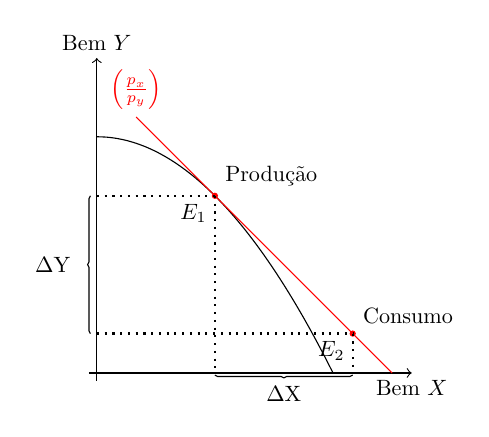
\begin{tikzpicture}[
			scale=1,
			every node/.style={scale=0.8},
			declare function = {fpp(\x) = 3 - (1/3) * \x^(2);},
			declare function = {tfpp(\x) = (15/4) - \x;}
			]

			\def\d{1.5}
			\def\e{3.25}

			\draw[->] (-0.1,0) -- (4,0) node[below] {Bem $X$};
			\draw[->] (0,-0.1) -- (0,4) node[above] {Bem $Y$};

			\draw[smooth,domain=0:3,variable=\x] plot (\x,{fpp(\x)});

			\draw[red,domain=0.5:(15/4),variable=\x] plot (\x,{tfpp(\x)});
			\draw[red] ({1/2},{tfpp(1/2)}) node [above] {$\left(\frac{p_x}{p_y}\right)$};
			\draw (\d,{fpp(\d)}) node[red,circle,fill,inner sep=1pt,label=above right:Produ\c c\~ao]{};
			\draw (\e,{tfpp(\e)}) node[red,circle,fill,inner sep=1pt,label=above right:Consumo]{};

			\draw[dotted, thick] (\d,{tfpp(\d)}) node[below left] {$E_1$} -- (\d,0);
			\draw[dotted, thick] (\e,{tfpp(\e)}) -- (\e,0);
			\draw[dotted, thick] (0,{tfpp(\e)}) -- (\e,{tfpp(\e)}) node[below left] {$E_2$};
			\draw[dotted, thick] (0,{tfpp(\d)}) -- (\d,{tfpp(\d)});

			\draw [decorate,decoration={brace,amplitude=1pt},xshift=-45pt,yshift=0pt] (\d,{tfpp(\e)}) -- (\d,{tfpp(\d)}) node [black,midway,xshift=-0.6cm] {$\Delta$Y};
			\draw [decorate,decoration={brace,mirror,amplitude=1pt},xshift=0pt,yshift=-15pt] (\d,{tfpp(\e)}) -- (\e,{tfpp(\e)}) node [black,midway,yshift=-0.3cm] {$\Delta$X};

			\end{tikzpicture}
		\end{column}
		\begin{column}{0.47\textwidth}
			{\scriptsize
			\begin{itemize}
				\item Termos de Troca no mercado: $\frac{p_x}{p_y}$
				\item Em $E_2$ verifica-se que: $$\Delta Y p_y + \Delta X p_x = 0$$
				\item Logo: $$\left|\frac{\Delta Y}{\Delta X}\right| =\frac{p_x}{p_y}$$
			\end{itemize}
			}
		\end{column}
	\end{columns}
\end{frame}

\begin{frame}
	\frametitle{Crescimento Econ\'omico}
	\begin{columns}
		\begin{column}{0.47\textwidth}
			\begin{tikzpicture}[
			scale=1,
			every node/.style={scale=0.8},
			declare function = {fpp1(\x) = 3 - (1/3) * \x^(2);},
			declare function = {fpp2(\x) = 3.5 - (1/3.5) * \x^(2);}
			]

				\draw[->] (-0.1,0) -- (4,0) node[below] {Bem $X$};
				\draw[->] (0,-0.1) -- (0,4) node[above] {Bem $Y$};

				\draw[smooth,domain=0:3,variable=\x] plot (\x,{fpp1(\x)});
				\draw[smooth,domain=0:3.5,variable=\x] plot (\x,{fpp2(\x)});

				\draw[->] (2,{fpp1(2)}) -- (2.4,{fpp2{2.4}});

			\end{tikzpicture}
		\end{column}
		\begin{column}{0.47\textwidth}
			\begin{tikzpicture}[
			scale=1,
			every node/.style={scale=0.8},
			declare function = {fpp1(\x) = 3 - (1/3) * \x^(2);},
			declare function = {fpp2(\x) = 3 - (1/3) * \x^(1.75);}
			]

				\draw[->] (-0.1,0) -- (4,0) node[below] {Bem $X$};
				\draw[->] (0,-0.1) -- (0,4) node[above] {Bem $Y$};

				\draw[smooth,domain=0:3,variable=\x] plot (\x,{fpp1(\x)});
				\draw[smooth,domain=0:3.5,variable=\x] plot (\x,{fpp2(\x)});

				\draw[->] (2.85,{fpp1(2.85)}) -- (3.3,{fpp2(3.3)});

			\end{tikzpicture}
		\end{column}
	\end{columns}
\end{frame}

\end{document}